\begin{figure}[ht]
  \centering
  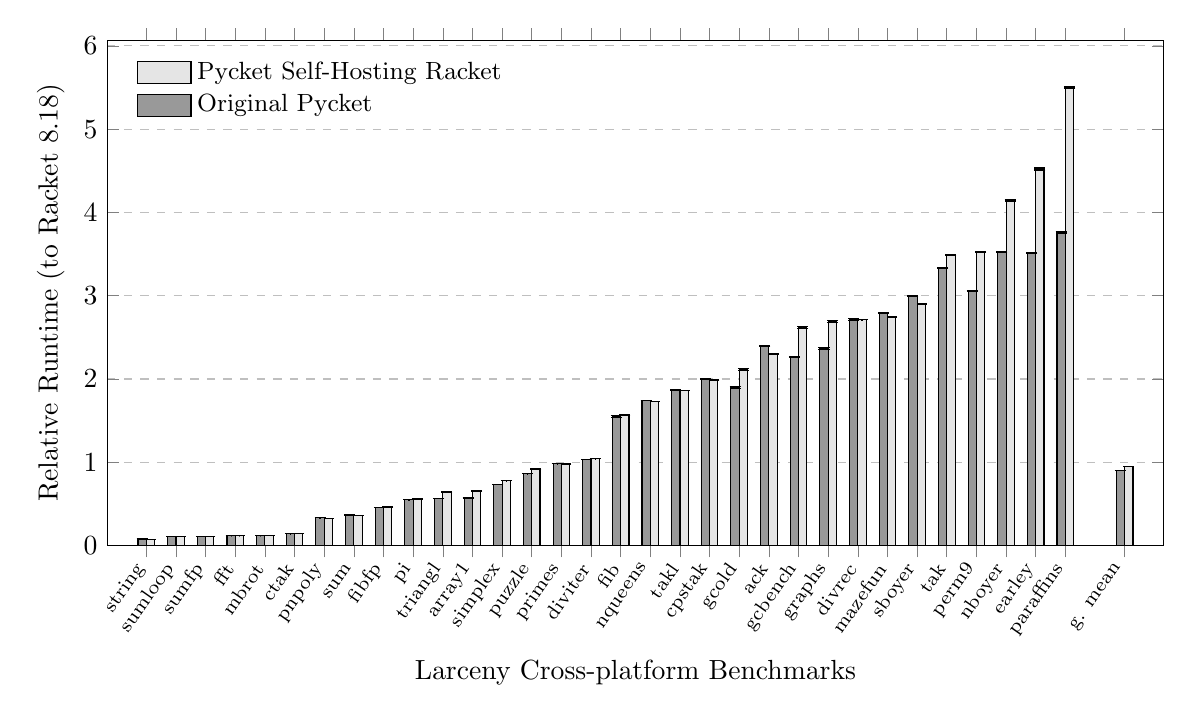
\begin{tikzpicture}
  \begin{axis}[
    ybar,
    bar shift=0pt,
    width=15cm,
    height=8cm,
    ylabel={Relative Runtime (to Racket 8.18)},
    xlabel={Larceny Cross-platform Benchmarks},
    symbolic x coords={string,sumloop,sumfp,fft,mbrot,ctak,pnpoly,sum,fibfp,pi,triangl,array1,simplex,puzzle,primes,diviter,fib,nqueens,takl,cpstak,gcold,ack,gcbench,graphs,divrec,mazefun,sboyer,tak,perm9,nboyer,earley,paraffins,,g. mean},
    xtick=data,
    xticklabel style={rotate=55,anchor=east,font=\scriptsize},
    ymin=0,
    enlarge x limits=0.04,
    ymajorgrids=true,
    grid style=dashed,
    legend style={
        at={(0.02,0.98)},
        anchor=north west,
        draw=none,
        fill=none,
        font=\small,
        /tikz/column 2/.style={anchor=west},
    },
    legend image code/.code={
        \draw[#1] (0,-0.14cm) rectangle (0.18cm,0.14cm);
    },
  ]
  % New Pycket With Warmup
  \addplot[
    ybar,
    fill=gray!20,
    draw=black,
    bar width=3pt,
    bar shift=+1.5pt,
    error bars/.cd,
      y dir=both,
      y explicit,
  ]
  coordinates {
    (string,0.07464) +- (0,0.000504)
    (sumloop,0.1103) +- (0,0.0000833)
    (sumfp,0.1142) +- (0,0.0000499)
    (fft,0.1179) +- (0,0.000209)
    (mbrot,0.1215) +- (0,0.000211)
    (ctak,0.1467) +- (0,0.000705)
    (pnpoly,0.3281) +- (0,0.000605)
    (sum,0.3622) +- (0,0.000208)
    (fibfp,0.4627) +- (0,0.000571)
    (pi,0.5596) +- (0,0.000879)
    (triangl,0.6441) +- (0,0.00105)
    (array1,0.6573) +- (0,0.00310)
    (simplex,0.7780) +- (0,0.00128)
    (puzzle,0.9170) +- (0,0.00197)
    (primes,0.9824) +- (0,0.00262)
    (diviter,1.045) +- (0,0.00116)
    (fib,1.567) +- (0,0.00247)
    (nqueens,1.731) +- (0,0.00272)
    (takl,1.862) +- (0,0.00346)
    (cpstak,1.986) +- (0,0.00227)
    (gcold,2.110) +- (0,0.0111)
    (ack,2.301) +- (0,0.00381)
    (gcbench,2.616) +- (0,0.00903)
    (graphs,2.690) +- (0,0.00929)
    (divrec,2.713) +- (0,0.00313)
    (mazefun,2.743) +- (0,0.00640)
    (sboyer,2.898) +- (0,0.00644)
    (tak,3.489) +- (0,0.00389)
    (perm9,3.520) +- (0,0.00489)
    (nboyer,4.141) +- (0,0.00855)
    (earley,4.521) +- (0,0.0115)
    (paraffins,5.505) +- (0,0.0109)
    (g. mean,0.9472) +- (0,0)
    };
  % Old Pycket With Warmup
  \addplot[
    ybar,
    fill=gray!80,
    draw=black,
    bar width=3pt,
    bar shift=-1.5pt,
    error bars/.cd,
      y dir=both,
      y explicit,
  ]
  coordinates {
    (string,0.08013) +- (0,0.000714)
    (sumloop,0.1102) +- (0,0.000110)
    (sumfp,0.1137) +- (0,0.0000706)
    (fft,0.1185) +- (0,0.000237)
    (mbrot,0.1196) +- (0,0.000133)
    (ctak,0.1427) +- (0,0.000525)
    (pnpoly,0.3361) +- (0,0.000739)
    (sum,0.3667) +- (0,0.000222)
    (fibfp,0.4595) +- (0,0.000743)
    (pi,0.5487) +- (0,0.000876)
    (triangl,0.5664) +- (0,0.000738)
    (array1,0.5729) +- (0,0.00209)
    (simplex,0.7339) +- (0,0.00103)
    (puzzle,0.8638) +- (0,0.00129)
    (primes,0.9851) +- (0,0.00113)
    (diviter,1.035) +- (0,0.00157)
    (fib,1.550) +- (0,0.00896)
    (nqueens,1.743) +- (0,0.00244)
    (takl,1.865) +- (0,0.00223)
    (cpstak,2.000) +- (0,0.00487)
    (gcold,1.895) +- (0,0.00998)
    (ack,2.396) +- (0,0.0105)
    (gcbench,2.261) +- (0,0.00435)
    (graphs,2.366) +- (0,0.0125)
    (divrec,2.713) +- (0,0.0156)
    (mazefun,2.798) +- (0,0.00524)
    (sboyer,2.995) +- (0,0.00478)
    (tak,3.331) +- (0,0.00413)
    (perm9,3.057) +- (0,0.0106)
    (nboyer,3.520) +- (0,0.00506)
    (earley,3.515) +- (0,0.00865)
    (paraffins,3.761) +- (0,0.00816)
    (g. mean,0.9005) +- (0,0)
    };
  \legend{Pycket Self-Hosting Racket, Original Pycket}
  \end{axis}
  \end{tikzpicture}
  \caption{Pycket with Self-hosting vs Original Pycket on Scheme benchmarks. Lower is better.}
  \label{fig:pycket-npww-opww-relR}
\end{figure}
